%------------------------------------------------------------------------------
% Template file for the submission of papers to IUCr journals in LaTeX2e
% using the iucr document class
% Copyright 1999-2013 International Union of Crystallography
% Version 1.6 (28 March 2013)
%------------------------------------------------------------------------------

\documentclass[preprint]{iucr}              % DO NOT DELETE THIS LINE

     %-------------------------------------------------------------------------
     % Information about journal to which submitted
     %-------------------------------------------------------------------------
     \journalcode{S}              % Indicate the journal to which submitted
                                  %   A - Acta Crystallographica Section A
                                  %   B - Acta Crystallographica Section B
                                  %   C - Acta Crystallographica Section C
                                  %   D - Acta Crystallographica Section D
                                  %   E - Acta Crystallographica Section E
                                  %   F - Acta Crystallographica Section F
                                  %   J - Journal of Applied Crystallography
                                  %   M - IUCrJ
                                  %   S - Journal of Synchrotron Radiation
\usepackage{graphicx}
%\graphicspath{ {./} }

\begin{document}                  % DO NOT DELETE THIS LINE

     %-------------------------------------------------------------------------
     % The introductory (header) part of the paper
     %-------------------------------------------------------------------------

     % The title of the paper. Use \shorttitle to indicate an abbreviated title
     % for use in running heads (you will need to uncomment it).

\title{New data analysis for BioSAXS at the ESRF}
%\shorttitle{Short Title}

     % Authors' names and addresses. Use \cauthor for the main (contact) author.
     % Use \author for all other authors. Use \aff for authors' affiliations.
     % Use lower-case letters in square brackets to link authors to their
     % affiliations; if there is only one affiliation address, remove the [a].

\cauthor[a]{Jérôme}{Kieffer}{jerome.kieffer@esrf.fr}{}
\author[b]{Martha}{Brennich}
\author[b]{Jean-Baptiste}{Florial}
\author[a]{Marcus}{Oscarsson}
\author[a]{Alejandro}{De Maria Antolinos}
\author[a]{Mark}{Tully}
\author[a]{Petra}{Pernot}
\aff[a]{The European Synchrotron, 71 Avenue des Martyrs, 38000 Grenoble \country{France}}
\aff[b]{European Molecular Biology Laboratory, 71 Avenue des Martyrs, 38000 Grenoble \country{France}}


     % Use \shortauthor to indicate an abbreviated author list for use in
     % running heads (you will need to uncomment it).

\shortauthor{Kieffer and Brennich}

     % Use \vita if required to give biographical details (for authors of
     % invited review papers only). Uncomment it.

%\vita{Author's biography}

     % Keywords (required for Journal of Synchrotron Radiation only)
     % Use the \keyword macro for each word or phrase, e.g. 
     % \keyword{X-ray diffraction}\keyword{muscle}

\keyword{BioSAXS; online data analysis; solution scattering; proteins; biological small-angle X-ray scattering; automation; high brilliance; structural biology;  high-throughput SAXS;  size-exclusion chromatography; online purification}

     % PDB and NDB reference codes for structures referenced in the article and
     % deposited with the Protein Data Bank and Nucleic Acids Database (Acta
     % Crystallographica Section D). Repeat for each separate structure e.g
     % \PDBref[dethiobiotin synthetase]{1byi} \NDBref[d(G$_4$CGC$_4$)]{ad0002}

%\PDBref[optional name]{refcode}
%\NDBref[optional name]{refcode}

\maketitle                        % DO NOT DELETE THIS LINE

\begin{synopsis}
Detailed presentation of the automatic data analysis pipelines for the BioSAXS beam-line at the European synchrotron.  
\end{synopsis}

\begin{abstract}
The second phase of the ESRF upgrade program did not only provide a new storage ring (EBS), it also allowed to refurbish several beam-lines, including the BioSAXS  BM29, which got a new wiggler source and a larger detector.
To cope with the resulting increased data-flux, analysis software needed to be rewritten to continue to ensure real-time processing.
This article describes \textit{FreeSAS}, an open-source collection of various SAXS analysis algorithms needed to reduce BioSAXS data, and \textit{dahu}, the tool used to interface data-analysis with beam-line control. 
It further presents the data processing pipelines for the different data acquisitions modes of the beam-line, using either a sample-changer for individual homogeneous samples or an inline size-exclusion chromatography setup.
\end{abstract}


     %-------------------------------------------------------------------------
     % The main body of the paper
     %-------------------------------------------------------------------------
     % Now enter the text of the document in multiple \section's, \subsection's
     % and \subsubsection's as required.

\section{Introduction}
Small angle scattering (SAS) provides information on the shape of macro-molecules on the nanometer scale and is particularly suited for biological samples thanks a large range of suitable buffer conditions.
Unlike single crystal diffraction or Nuclear magnetic resonance (NMR) which offer atomic resolution, bioSAXS provides only information on the envelope of macro-molecules: it allows to validate the relative position of large structures and the assembly of biological complexes \cite{biosaxs_rev2018}. 
Structural biologists perform SAXS experiments to validate the size and the shape of their protein or complex under study. 
Since most beam-line users are neither synchrotron, nor SAXS specialists, a fully automated analysis of their data is of crucial importance for them. 
Automated data analysis should provided them not only with the reduced and pre-analyzed data, but also with all metadata and parameters needed to get their results published according to the relevant guidelines \cite{guidelines_2017}.
These metadata are also important to reprocess data using third party software to ensure comparable results. 

The BioSAXS beam-line from the European synchrotron \cite{BM29paper} had an automated pipeline for the data-analysis which was based on \textsc{edna} \cite{edna} and was using the \textsc{atsas} \cite{ATSAS2} software underneath. 
While the outcome of the processing was very appreciated by beam-line users, the system was already close to the maximal throughput possible in terms of performances. 
The new EBS source \cite{EBS} of the ESRF not only provides a higher brilliance, but also new wiggler sources for the former bending-magnet beam-lines which triggered the re-build and the upgrade of most of them. 
The BioSAXS beam-line (BM29) has been rebuilt in 2019 and features a 2-pole wiggler and a new Pilatus3 2M detector (previously 1M) planned to be mounted in vacuum. 
This has lead to a substantial increase of data-rate; mainly due to the new detector, twice larger than the former one. 

This paper is divided in two main parts, starting with a presentation of the tools used for 
processing SAS data (\textit{FreeSAS}) and for assembling pipelines (\textit{dahu}).
Then three different pipelines are presented: a common one used for the reduction of the scattering images and two dedicated: one for sample-changer-based experiments (referred as SC) and another one dealing with chronological data used with the size exclusion chromatography experiments (referred as \textsc{hplc}).

\section{Tools}

To meet the real-time data analysis requirements, all software used at the beam-line has been upgraded.
Precise benchmark of the execution times of the previous \textsc{edna}-based pipeline demonstrated that 
most time was spent in launching external tools coming from the \textsc{atsas} suite and in parsing text files produced by those tools.
It was decided to rewrite all pipeline in plain Python \cite{python} and call SAS-related tasks from a library, \textit{FreeSAS}. 
Finally this code is interfaced to the control software, \textsc{bliss} \cite{bliss}, via Tango \cite{tango} and uses a simple task scheduler, \textit{dahu}, already used in production on the TruSAXS beam-line \cite{id02_2022}.

\subsection{Small angle scattering analysis tools, \textit{FreeSAS}}

\textit{FreeSAS} is a Python library containing SAS-analysis tools available both via command line interface and from a Python API. 
It does not claim to be as complete as the \textsc{atsas} counterpart \cite{ATSAS3},
but is free, released under the MIT license (i.e. it can be included in commercial products), all source code is available publicly on github \cite{freesas} and
open to external contributions.
Despite Python being an interpreted language, FreeSAS is performance oriented and most of the processing is performed with Cython \cite{cython} extensions written in C to obtain the required performances. 
\textit{FreeSAS} has been made available and packaged independently from \textit{dahu} (the online analysis tools) so that scientists can reprocess their data and compare their results with those of other analysis software. 
The latest release, \textit{FreeSAS} 0.9, supports Python 3.6 to 3.9.

\subsubsection{SAS plotting:} The \textit{freesas} tool (figure \ref{plot}) provides a way to plot  a semi-logarithmic representation the SAS curve: $I=f(q)$, where $q = 4\pi sin(2\theta/2)/\lambda$ is the amplitude of the scattering vector, $\theta$ is scattering angle, $\lambda$ wavelength and $I$ the recorded intensity at a given $q$, along side some basic analyses which are described in the next sections.

\begin{figure}
\label{plot}
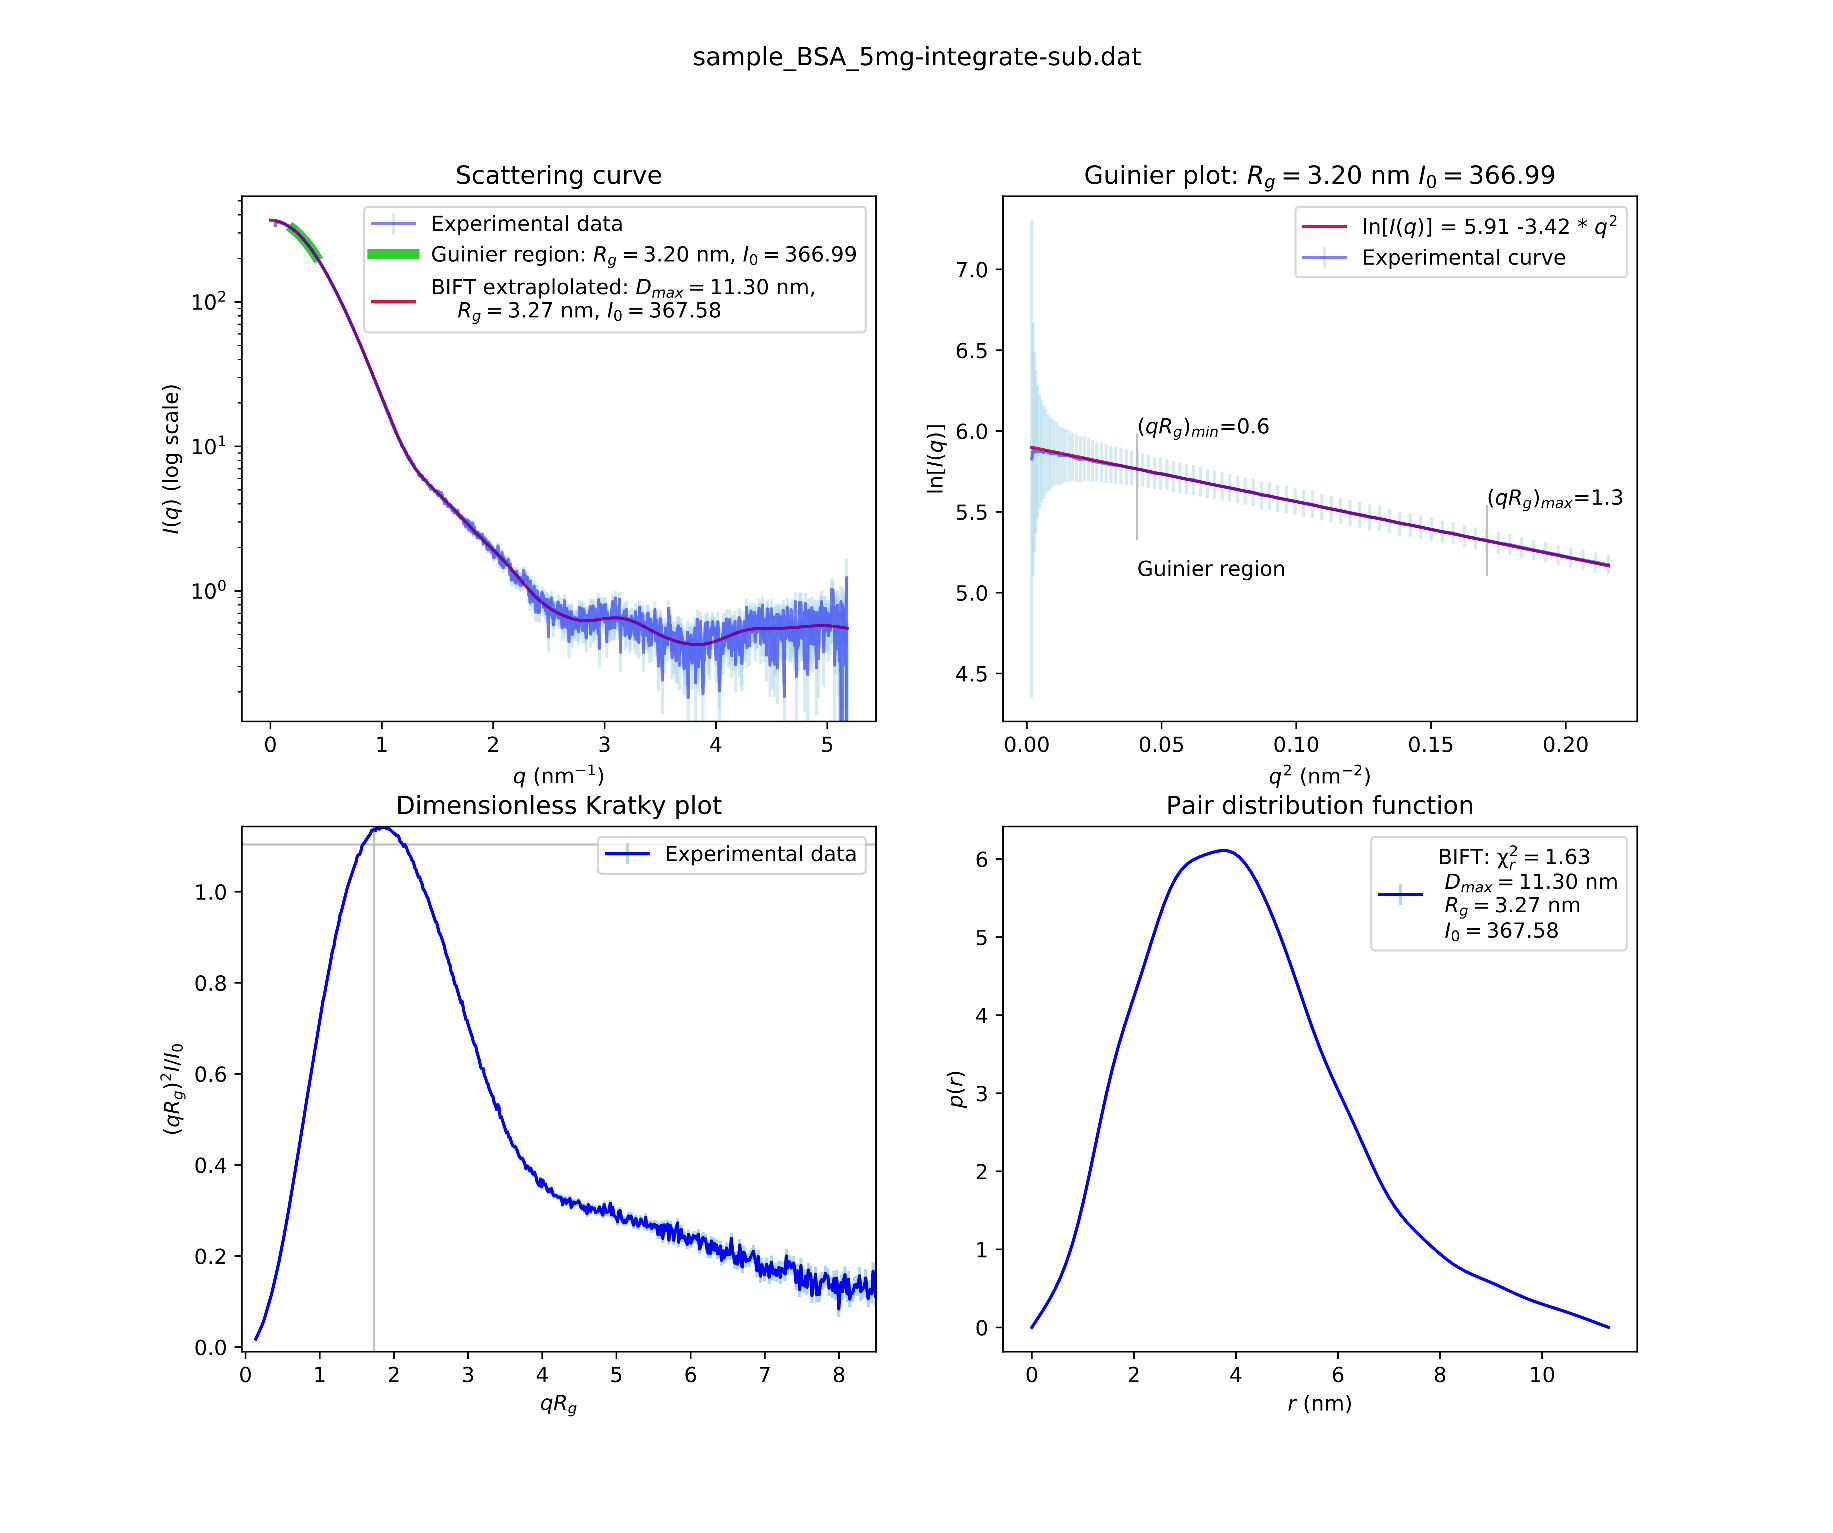
\includegraphics[width=12cm]{Figure_1.eps}
\caption{Default visualization of bioSAS data with automated analysis using \textit{freesas}}
\end{figure}

\subsubsection{Guinier-region fitting:}
The first analysis performed on bioSAXS data determines the radius of gyration ($R_g$) of the solvated macro-molecule and the forwards scattering intensity, $I_0$ \cite{guinier}.
Based on the Tailor expansion of the scattering curve at $q=0$, $R_g$ is obtained from the the linear regression of $log(I(q)) = log(I_0)-1/3 (R_{G}q)^{2}$ on the proper q-range at small angles, called the Guinier Range.
The selection of the Guinier-region is far from being obvious due to the beam-stop shadow, aggregation effects, and its upper limit depends on $R_g$ itself: $q \cdot R_g<1.3$.
Thus multiple implementation are provided: \textit{autorg}, which derives from the implementation in BioXTAS-RAW \cite{bioxtasraw}; \textit{auto-guinier}, which searches for a consensus region rather than the best possible Guinier-region; and finally \textit{auto-gpa}, which performs a Guinier-peak-analysis \cite{gpa}. 
The later is a quick assessment of the $R_g$ and $I_0$, sometimes less robust than the two other implementations, but suitable when many datasets are to be analyzed like in chromatography mode.
It is worth mentioning that none of the three algorithms provide the exact same results as the original \textsc{autorg} \cite{ATSAS2} version from \textsc{atsas}. 
This highlights the importance of publishing the actual implementation of the algorithms with the associated numerical parameters used in it.
  
\subsubsection{Pair distribution function:}
Although the scattering curve $I(q)$ is the Fourier transform of the pair distribution function $p(r)$, the later cannot directly be obtained from an inverse Fourier transform (IFT) due to the loss of phase information and the limited amount of information in the scattering curve. 
This ill-posed mathematical problem has no exact solution and is usually inverted with some extra constraints imposed, like the finite size of the support (defined by the maximum diameter, $Dmax$).    
FreeSAS proposes an IFT based on the Bayesian statistics and derived from BIFT \cite{bift}, like the one found in \citeasnoun{bioxtasraw}.
%The command-line program to perfrom and IFT is \textit{bift.py}. 
Despite different approach, the result of \textit{bift} is similar to the \textsc{datgnom} \cite{ATSAS1} from \textsc{atsas} which uses a Tikhonov's regularization.
The diameter found, $Dmax$, is directly comparable with the one provided by \textsc{atsas}, but the parameter $\alpha$ differs since the theory used for regularisation differs. 

\subsubsection{Assessment of equivalence of scattering curves: }
To obtain the best possible signal from the sample, the capillary containing flowing solution is exposed multiple times with a short exposure.
All equivalent frames are then merged to optimized the signal/noise ratio without pollution from radiation damaged data.  
The equivalence of a couple of frames is obtained from the correlation-map (CorMap) algorithm implemented from the publication by \citeasnoun{CorMap}.

\subsubsection{Overlay of bead models:}
\textit{subpycomp} \cite{BM29ODA}, a tool to rotate/flip bead models and overlay them prior to merging them. It is equivalent to the \textsc{supcomb} \cite{supcomb} tool from \textsc{atsas}. 

\subsubsection{Extraction to ASCII data:} with the increased frame-rate of the new beam-line, the historical 3-column text file with $q$, $I_{avg}$, $\sigma(I)$ became unpractical and has been superseded by the hierarchical-data format, HDF5 \cite{hdf5} which contains all analysed data derived from raw data.
The \textit{extract-ascii} tool is designed to generate text files in the  $q$, $I_{avg}$, $\sigma(I)$ format and offer a compatibility with third-party tools.

\subsection{The job-manager: \textit{dahu}}

The role of the job manager is to ensure all processing requested by the client (i.e. the user interface) are actually performed, informs the client about the finished jobs and warns it in case of an error.
%(what do you mean by client? The requestor?) is informed in case of issues. %Only if issues arrise? Or is other information also returned?
%This subsection is purely technical and can be skipped. 

\textsc{edna} was used as workflow manager for the previous data-analysis pipeline for many protein crystallography beam-lines \cite{edna} and for the BioSAXS beam-line at the ESRF \cite{BM29ODA}.
The parallelization model used in \textsc{edna} is based on Python threads and forking processes which was wasting resources in serializing and inter-process communication. 
%Despite the Global Interpreter Lock (GIL) which prevents Python from running multiple threads simultaneously, parallel processing occues when the work is performed in separated process. 
%This implies that for each task to be perfomed, an input file needs to be written before launching the process and the result file needs to be read and parsed after the end of the processing.
%When processing was doing loops of jobs, most of the time was spent in string manipulation for writing and parsing strings (for example: to compare pair-wise 10 frames it takes 45 process to be launched !)
 
The \textit{dahu} job-manager was designed for the TruSAXS beamline \cite{id02_2022} with those limitation in mind. 
%Text manipulation was simplified by switching from XML to JSON data-structure representation. 
%This modification alone has proven to speed up \textsc{edna} by a factor 3 !
The tango interface \cite{tango} was kept similar to the one in \textsc{edna} to ease the adoption.
%, the adaptation was  framework were kept and the code was simplified to the extreme since \textit{dahu} represents only 1000 lines of code. 
The scheduling of jobs is performed via a shared queue and only few worker are running simultaneously in threads.
Thus the code runs actually in parallel only in sections where the Global Interpreter Lock from Python (GIL) is released, like in Cython extensions \cite{cython} from FreeSAS or in the OpenCL code from pyFAI \cite{pyFAI_gpu}.

\subsubsection{Dahu-jobs}
manage the execution of the \textit{plugins} (see here-after), provide an unique identifier which gives access the status and output of the processing.
Jobs see their input and output saved to the disk, this allow off-line reprocessing in case of issue during online data-analysis.

\subsubsection{Dahu-plugins} implement the processing logic of the different pipelines.
Written in simple Python and fairly independent from the \textit{dahu} framework, those plugins are often written or modified by beam-line scientists themselves.

\subsubsection{Offline re-processing}
is made possible by the \textit{dahu-reprocess} command-line tool.
This tool was designed to (re-)execute one or several jobs based on the description saved by the online data analysis server. 
Since \textit{dahu} has virtually no dependencies, it can be deployed on any computer to reprocess data. 
Nevertheless, to reprocess data acquired at the BioSAXS beam-line, one would need FreeSAS and all the other dependencies of BioSAXS \textit{plugins}, which are all documented, publicly available and all open-source.

\section{Data analysis pipelines}
\label{pipeline}
There are two main experiments performed at the BioSAXS beam-line, either using the sample changer or the inline-chromatography setup (\textsc{hplc}).
Thus, two analysis pipelines were built, one for each of those experimental mode.
The common part, mainly dealing with azimuthal integration, got integrated into a pre-processing pipeline called \textit{integrate multi-frame}.
%This would profit from  description of how the data is actually structured in the two acquisition modes. I got completely lost here!

Since the Pilatus 2M detector is controlled by the \textsc{lima} software \cite{lima}, raw images are saved in a HDF5 file-format \cite{hdf5} with ten or hundred frames per file (depending on the acquisition mode, figure \ref{lima}).
HDF5 offers compression, faster data-access, symbolic links to datasets from one file to another ... but it is dramatically different from the former pipeline which was triggered frame per frame.

\begin{figure}
     \caption{Layout of a raw image HDF5-file produced by the \textsc{lima} acquisition software, visualized with the \textit{silx} viewer.}
     %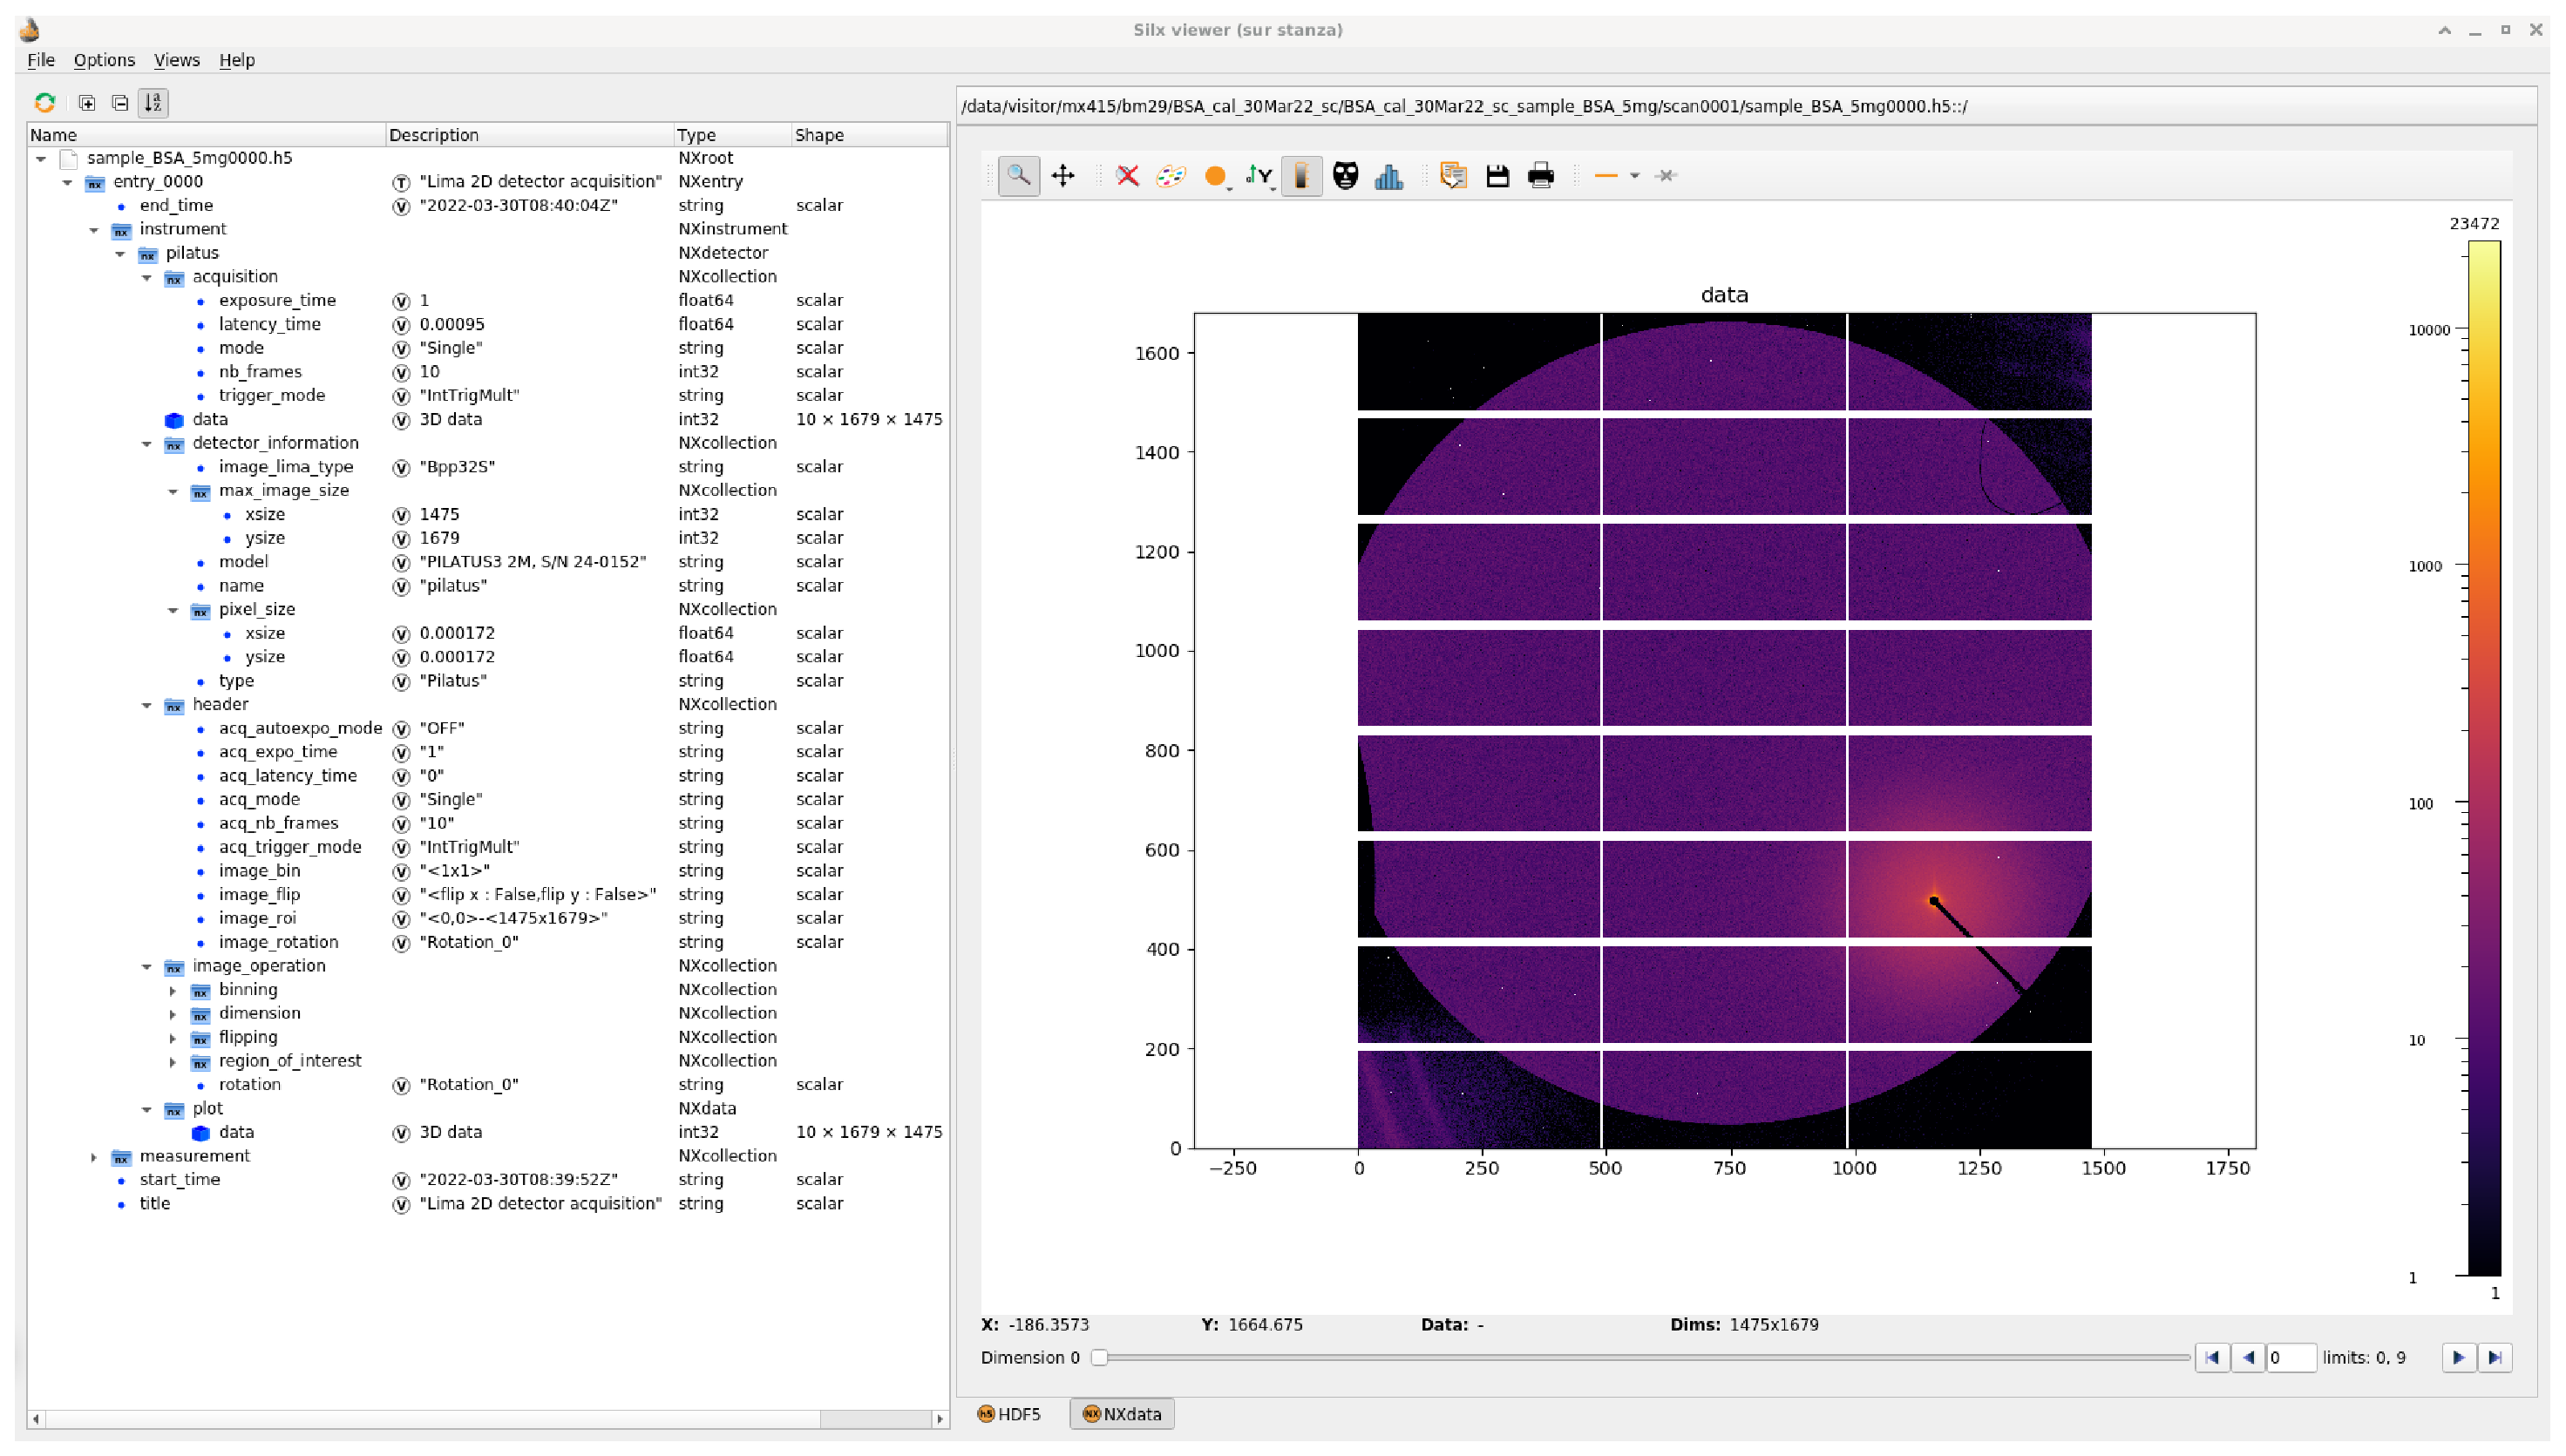
\includegraphics[width=12cm]{lima.eps}
     \includegraphics[width=12cm]{Figure_2.eps}
     \label{lima}
\end{figure}

ESRF provides several tools to visualize those HDF5 files like \textit{silx view} \cite{silx} which is a graphical user interface based on Qt \cite{pyqt} or the web-viewer \textit{h5web} \cite{h5web} to visualize those files inside a web-browser.
This \textit{h5web} is already used in the beam-line control user interface BsxCuBE3 \cite{bm29_2022} and will be used in the new ISPyB interface (under development).
\textsc{lima} files (figure \ref{lima}) contain no metadata beside the camera configuration.
Thus all sample and experiment description (geometry, mask, \ldots), beam-stop diode intensities and other processing parameters have to be provided by the experiment sequencer, \textsc{bliss}, as part of the job description when triggering the process.

The versatility of the HDF5 format allows to have one single output file for all results produced by a processing pipeline, making backup easier.
Each pipeline registers the result of every individual processing step of the pipeline in the output HDF5 file (as HDF5-groups), together with the configuration associated with the processing.
Input datasets are referenced using external links, which avoids data duplication while keeping traceability. 
Finally metadata describing the sample, its buffer and the configuration of the beam-line are also recorded using the Nexus convention \cite{nexus}.
Each processing pipeline defines a default plot which tries to summarize the experimental result to the user.

\subsection{Multi-frame integration pipeline}
\label{multiframe_pipeline}
The multi-frame integration pipeline is triggered with the name of one \textsc{lima}-file (containing several frames) and all additional metadata describing the sample and the experiment.
All other processing parameters are sent in the same way, regardless if they are read from the user-interface or collected by \textsc{bliss}.

\begin{figure}
     \label{multiframe_worflow}
     \begin{center} 
     \caption{Schematic of the multi-frame integration pipeline: 
     1. azimuthal integration of individual frames; 
     2. comparison of 1d-curves;
     3. equivalent frames are averaged;
     4. azimuthal integration of the averaged image.}
     %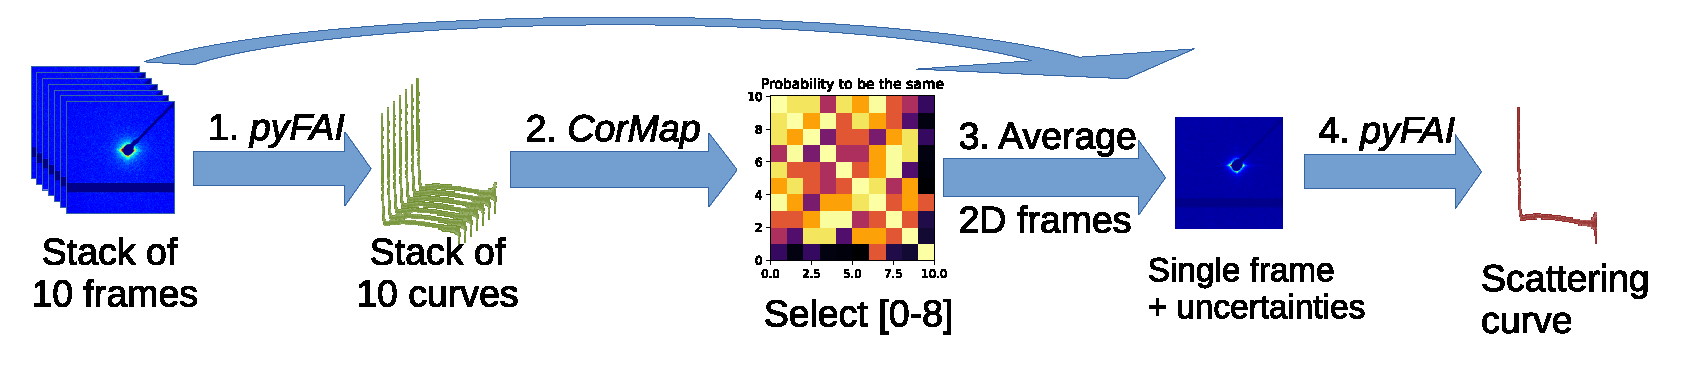
\includegraphics[width=12cm]{multiframe_pipeline.eps}
     \includegraphics[width=12cm]{Figure_3.eps}
     \end{center}
\end{figure}

The figure \ref{multiframe} presents a file produced by this processing pipeline with the default plot consisting in the semi-logarithmic representation of the scattering curve $I(q)$ viewed with \textit{silx}.
This pipeline is built of four subsequent analysis steps, as illustrated in figure \ref{multiframe_worflow}:
\begin{enumerate}
\item Each recorded image is azimuthally integrated with \textit{pyFAI} \cite{pyfai_2020} to produce one scattering curves per frame;
\item Scattering curves are compared, searching for radiation damage using the \textit{CorMap} algorithm \cite{CorMap}; the probability for each pair of curves to be the same is compared to thresholds to assess their equivalence, those thresholds depend if frames were adjacent or not;
\item Equivalent images are averaged pixel-wise, weighted by the beam-stop diode intensity; variance is assessed using Poisson law;
\item The averaged frame is finally azimuthally integrated and uncertainties propagated accordingly. 
\end{enumerate}

\begin{figure}
     \caption{Layout of a HDF5-file obtained from the multi-frame integration pipeline, visualized with the \textit{silx} viewer.
     On the left-hand side, one can recognize in the HDF5-tree the structure of the pipeline described figure \ref{multiframe_worflow}.
     The right-hand side presents the scattering curve of BSA before subtraction of background signal.}
     %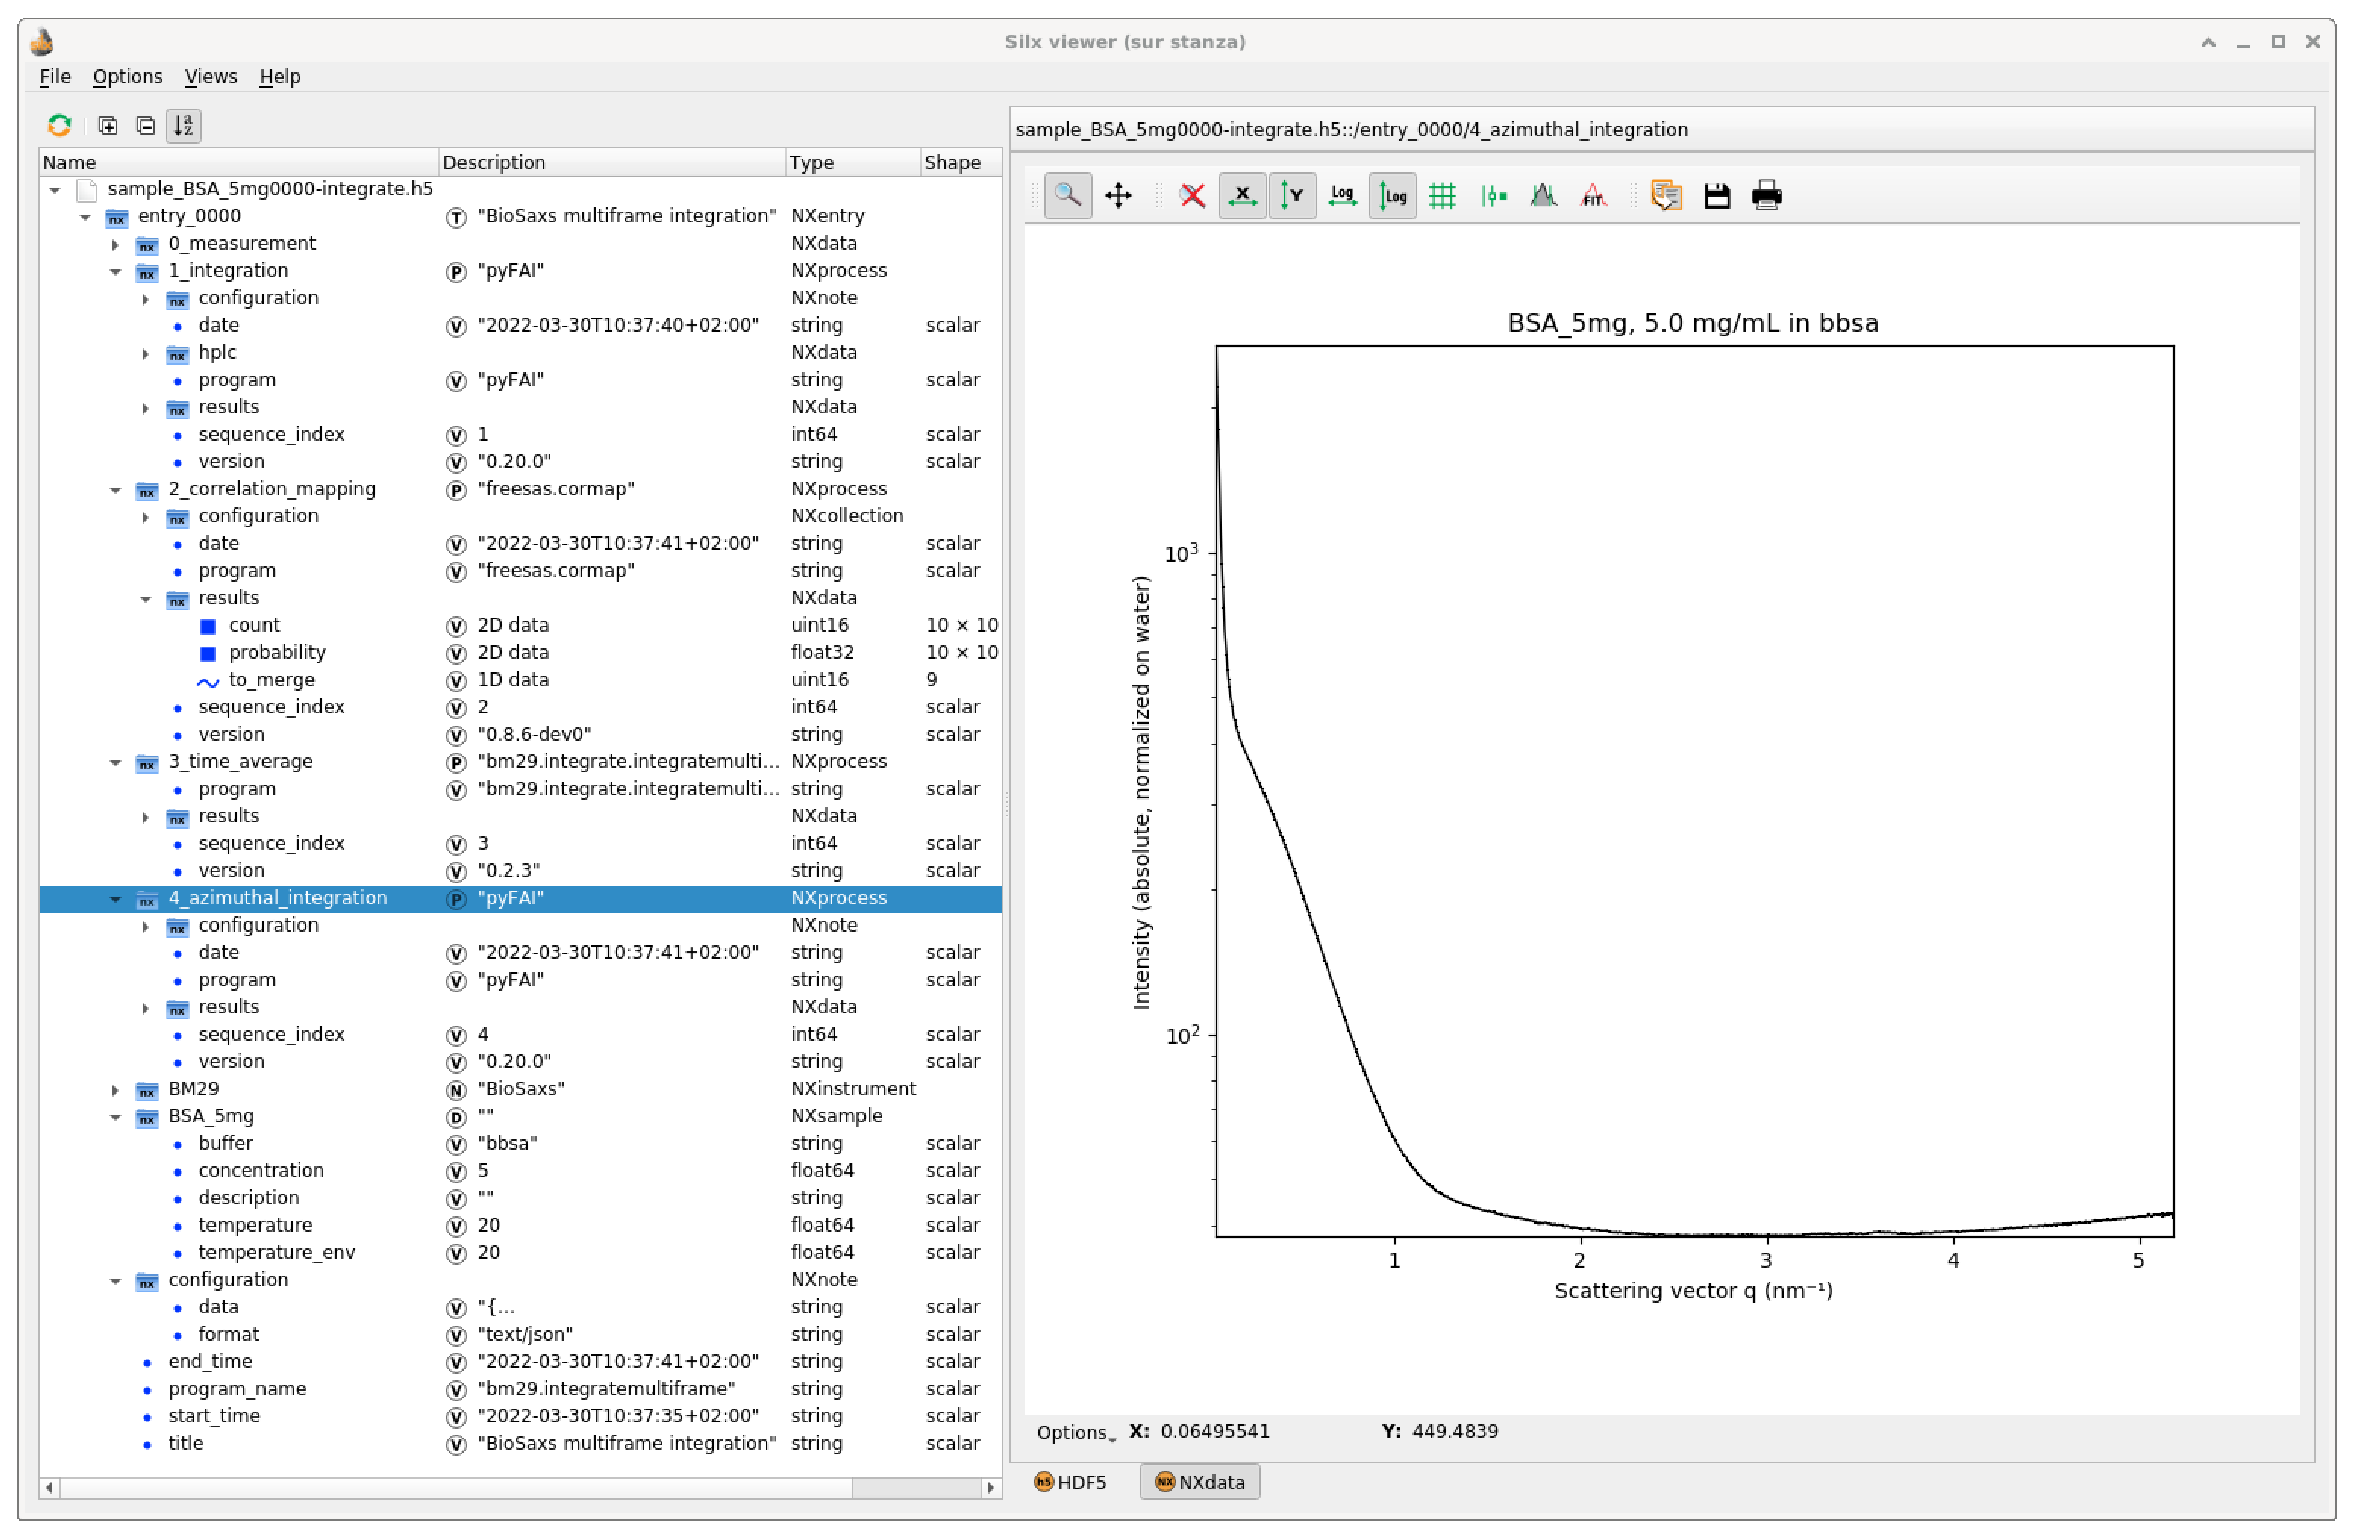
\includegraphics[width=12cm]{multiframe.eps}
     \includegraphics[width=12cm]{Figure_4.eps}
     \label{multiframe}
\end{figure}

The plot of the azimuthally integrated averaged frame (at stage 4) is set as the default display  when processing data in sample-changer mode.
In \textsc{hplc}-mode, the default plot represents the summed intensity as function of time, which is a fraction of the complete chromatogram. 
The HDF5-file additionally includes external links to the raw frames as acquired by the detector (stage 0).
%Uncertainties on pixel intensities are assumed to be Poissonian and propagated accordingly.
%Azimuthal integration is a common reduction step for all small angle scattering experiments. 
%The BioSAXS beamline uses \textit{pyFAI} \cite{pyfai_2020} as core of its \textit{multiframe} integration pipeline.
%Thanks to the GPU-computing, \textit{pyFAI} is able to integrate each frame within a millisecond.
%In order to avoid cross-correlation between neighboring bins, pixel splitting is disabled.
%Frames are read from the HDF5 file produced by \textit{LImA} \cite{lima} and all other metadata like the sample description and the transmitted  intensity (recorded on the beam-stop diode) are sent as part of the job description from BsxCuBE3, the graphical user interface running the beamline.

%In sample changer mode, all frames are expected to be similar and needs to be merged, except the ones exhibiting radiation damage which should be discarded.
%For this, every single scattering curve is compared with all others to build the correlation-map \cite{CorMap}. 
%This map allows to determine the largest group of frames which are equivalent based on two threshold, the minimum probability for two adjacent frames to be the same and the threshold for frames which are not adjacent. 

%Frames found equivalent in the correlation-map analysis are averaged taking into account normalization from the beam-stop diode value. 
%The uncertainties for pixel values is propagated assuming Poisson statistics. 
%The standard deviation of each pixel in the stack of equivalent frames was found noticably lower than the propagated variance, assuming a Poisson statistic.
%The averaged frame (with its associated uncertainties) is finally azimuthally integrated with pyFAI and stored in the output file. 
%The SAXS plot $I = f(q)$ is set as the default representation of this output file.

%In chromatography mode, the acquisition occurs typically over half an hour representing thousand images at 1Hz acquisition rate. 
%This results in several HDF5-files containing partial chromatograms.
%The total scattering is computed by summing all intensities in each of the curve to build a simple chromatogram $I_{sum} = f(t)$ 
%which indicates weather a sample eluted from the chromatography column or not. 
%This (partial) chromatogram is the default plot for this type of integrated file.

It is worth mentioning that time-averaging and azimuthal-integration are not (strictly) commutative as demonstrated in appendix \ref{rational}, especially when it comes to uncertainty propagation.


\subsection{Sample-changer pipeline}
\label{sc-pipeline}
In sample-changer mode, solution containing samples are acquired alternatively with pure buffer solutions.
The throughput of the beam-line is then limited by the pipetting system of the robot and the delay for cleaning the exposure chamber.  
The processing is triggered with integrated data from the sample (i.e. the name of the file containing the sample data after azimuthal integration) and a list of 
buffer files corresponding to the different acquisition of buffers, usually the buffer before and the buffer after the sample acquisition.

\begin{figure}
\label{samplechanger_worflow}
\includegraphics[width=12cm]{Figure_5.eps}
%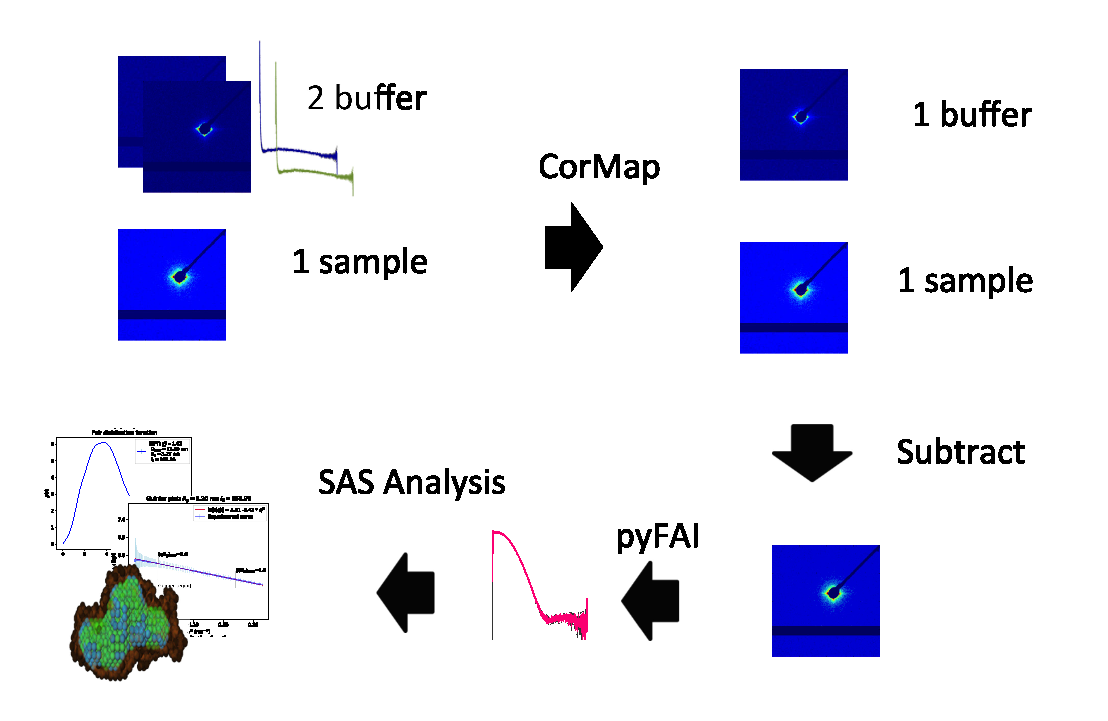
\includegraphics[width=12cm]{samplechanger_pipeline.eps}
\caption{Schematic of the sample-changer pipline: 
1. Comparison of buffer frames image;
2. Subtraction of averaged buffer image from sample image;
3. Azimuthal integration the background subtrated image;
4. and subsequent: SAS analysis, including Guinier, Kratky and BIFT analysis.}
\end{figure}

The sample-changer pipeline is schematized in figure \ref{samplechanger_worflow} and produces a new HDF5-file with the subtracted data in it, such file is visualized in figure \ref{subtracted} and contains the results of this 8-stage pipeline: 
\begin{enumerate}
    \item Comparison of buffer curves using the \textit{CorMap} algorithm \cite{CorMap};
    \item Buffer frames are averaged together and subtracted from the sample averaged frame (i.e. still in 2D);
    \item Azimuthal integration of the subtracted frame with \textit{pyFAI} \cite{pyfai_2020};
    \item Guinier analysis with the associated linear regression of $log(I(q))$ vs. $log(I_0)-1/3 (R_{G}q)^{2}$ at low $q$ as default plot;
    \item Dimensionless Kratky plot: $(q\cdot R_g)^2\cdot I/I_0$  vs. $q\cdot R_g$;
    \item Porod \cite{glatter+kratky} and Rambo-Tainer invariant \cite{RamboTainerNature2013} calculation to assess the the molecular volume and molecular mass of the sample;
    \item Indirect inverse Fourier transform using the BIFT algorithm \cite{bift} provides the pair distribution function $p(r)$;
    \item Transfer of reduced data to ISPyB for BioSAXS (compatibility layer with legacy ISPyB).
\end{enumerate}
As in the \textit{multi-frame} processing pipeline (\ref{multiframe_pipeline}), there is a link to the source data as stage zero of the processing to ensure a perfect tracking of the experiment.
The pair distribution function obtained from BIFT (stage 7) allows to calculation of the radius of gyration in real space and should confirm the radius of gyration found from Guinier fit (stage 4). 

\begin{figure}
\label{subtracted}
%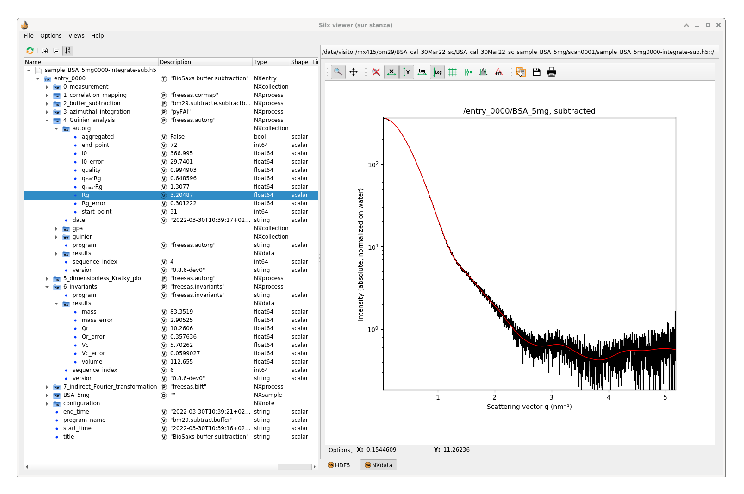
\includegraphics[width=12cm]{subtracted.eps}
\includegraphics[width=12cm]{Figure_6.eps}
\caption{Default visualization of the HDF5-file produced by the sample changer pipeline with the \textit{silx} viewer. 
The superimposed red curve corresponds to the BIFT modeled data.}
\end{figure}



%Integrated buffer data are compared with the correlation-map algorithm in order to validate that acquired buffer matches, 
%If they don't, only the buffer acquires prior to the sample acquisition is considered
%Averaging of the buffer signal and subtraction of the buffer from sample data are both performed on the 
%2D frames. 
Once again, the subtraction is made on 2D frames and not on integrated curves for similar reasons as the one presented in appendix \ref{rational}.

%Working on the 2D data frames allows a better preservation of weak signals and cancels-out systematic deviation from certain pixels.
%!! 
%this statemern needs prrof, either by citation or by showing some statistics comparing the estimated standard deviation for same data (water? BSA?) for both the old and new pipelines.
%!!
% The subtracted frame is then integrated using \textit{pyFAI} and the associated uncertainties propagated according to \cite{pyfai_2020}.

% The subtracted SAXS curve is then analyzed with Guinier fit (all three algorithms available in FreeSAS are tested)
% to provide the hydrodynamic radius of gyration, $R_g$ and the forwards scattering intensity $I_0$.
% A dimensionless Kratky plot provides some assessment on the complicity of the sample,  or if it is unfolded. 
% Finally, the inverse Fourier is obtained from BIFT and provides the diameter $D_{max}$, the pair-distribution 
% and confirms the radius of gyration.
% After the analysis, the volume is calculated from the Porod formula, and the Rambo-Tainer invariants provide  information about the molecular weight of the sample.
% All those information are registered and the default plot is defined to have a display similar to figure \ref{subtracted}
% with the scattering curve superimposed with the BIFT-fitted scattering curve.

The final stage of this pipeline is to register those results into the ISPyB for BioSAXS database \cite{ISPYBB} (https://exi.esrf.fr), and instantly made available to the user via the data portal (https://data.esrf.fr). 
The same data are shared with the BsxCuBE3 control software via a memcached key-value database for instant feed-back.

\subsection{SEC-SAXS pipeline}
%I have to admit that I ma quite lost in this section. I suspect the reason is that I do not understnad how the input data looks like? Are there 10 partial chromatograms per run? 100? 1000? that makes quite a difference, doesn't it? 
Online purification of the sample allows to reduce the effect of oligomerization.
It has become a standard procedure since it was introduced to BM29 in 2012 \cite{SECPaper2012} and accounts now for two third of all measurements performed at the beam-line.

In this mode, a typical acquisition consists of one thousand frames acquired at one frame per second.
Those data are saved as ten files containing each one hundred frames.
The input for this pipeline a list of HDF5-files with partial chromatograms integrated by the \textit{multi-frame} pipeline presented in section \ref{multiframe_pipeline}. 
%How large is such ar partial chromatogram? How many are there? How is their size decided?
The \textsc{hplc} pipeline, figure \ref{hplc_worflow}, re-builds the complete chromatogram and performs the complete analysis of the different fractions, taking into account the possibility for empty sections (due to missing input files).
This pipeline produces files which are presented in figure \ref{hplc}.
\begin{figure}
\label{hplc_worflow}
%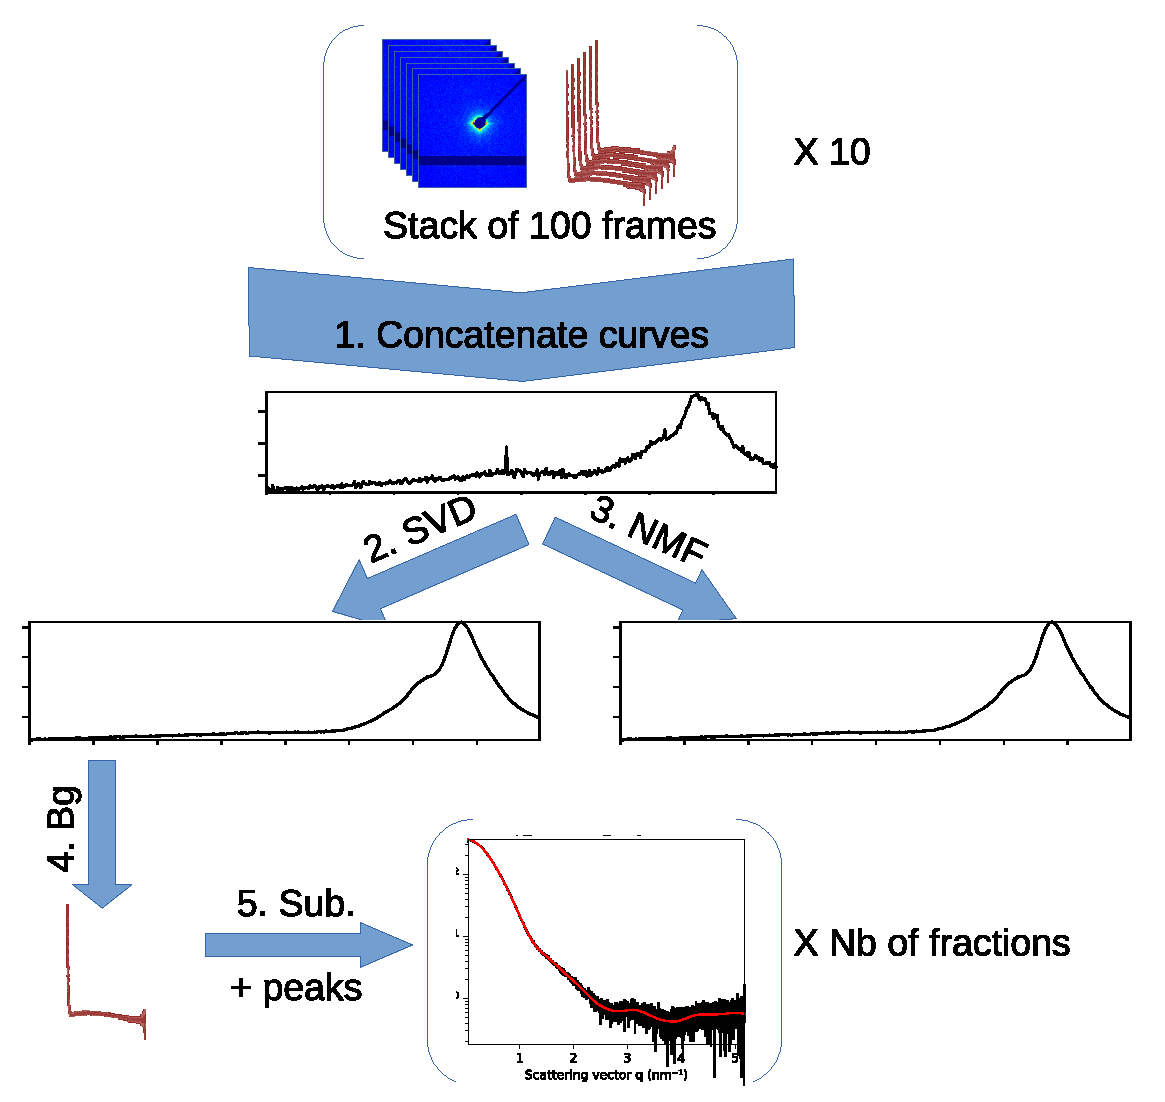
\includegraphics[width=12cm]{HPLC_pipeline.eps}
\includegraphics[width=12cm]{Figure_7.eps}
\caption{Schematic of the \textsc{hplc} pipline: 
1. Concatenate ;
2.\&3. Multivariate analysis;
4. Background extraction;
5. Peak finding
6. SAS analysis on each fraction}
\end{figure}

This chromatography pipeline has six stages:
\begin{enumerate}
    \item Concatenate partial chromatograms (1D curves) provided by the \textit{multi-frame} pipeline to obtain the full chromatogram; Empty/missing regions are handled here;
    % TO obtain what? All individual frames? All averages frames?
    \item Perform a Singlar Value Decomposition (SVD) on the chromatogram to assess the number of components and extract scattering from the the background; 
    %on the completety, non-background corrected chromatogram?
    \item Perform a non-negative matrix factorisation (NMF) to get an idea of the scattering curve of the different fractions; 
    \item Select points belonging to the background by comparing experimental scattering with the first singular-vector from the SVD; average-out selected curves; %If understand the following correclty, it is simply the first 30 \%? is there are reason this is not dome before SVD and NMF
    \item Perform peak-picking on subtracted curves; analyse each fraction with a similar pipeline to the one presented in \ref{sc-pipeline} %Where do those fractions  come from?
    \item Prepare the data and send them to ISPyB for BioSAXS.
\end{enumerate}

\begin{figure}
\label{hplc}
\begin{center}
\includegraphics[width=12cm]{Figure_8.eps}
%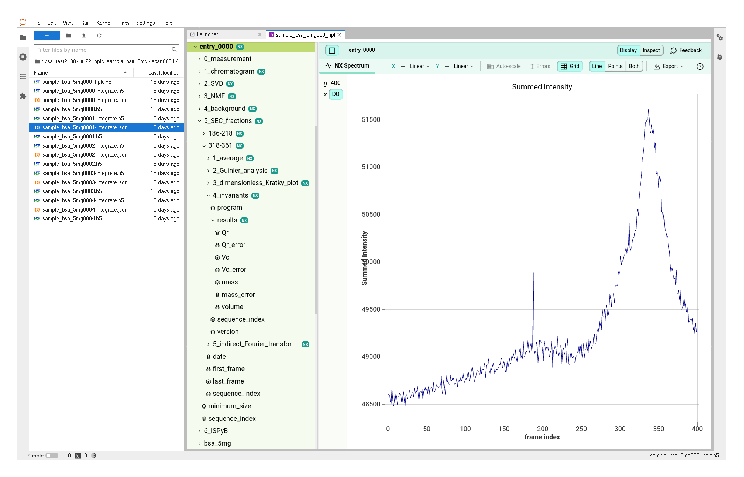
\includegraphics[width=12cm]{HPLC-h5web.eps}
\caption{Default visualization of the HDF5-file produced by the \textsc{hplc} pipeline with the \textit{h5web} viewer integrated into JupyterLab.}
\end{center}
\end{figure}

Multivariate analysis is performed to extract the signal of the macro-molecule from background scattering, and provide a hint on how many components have been separated in the chromatography.
\citeasnoun{svd_threshold} provides the number of singular values/vectors which are to be saved after the SVD decomposition
The SVD is provided by the NumPy package \cite{numpy}.   
The first singular vector contains mainly background scattering, the following ones contains signal from the separated components and subsequent ones account only for noise.
Since SVD (provided by NumPy \cite{numpy}), does not enforce positivity of extracted singular vectors, a NMF decomposition is performed (provided by scikit-learn \cite{sklearn}).
%This decomposes the chromatogram $I(q)$ as a serie of singular-values representing the chromatogram for every component stored in the associated singular-vector. 
%There are as many singular values/vectors pairs as time-steps acquired in the experiment but only the few firsts account for actual signal.
% The elution of the sample is usually very visible in the chromatogram associated to the second and third singular values.

%Unlike SVD, the NMF factorisation is neither fast, nor unique and the number of component needs to be known in advance.
%Five component are extracted by default, accounting for a two solvent mixture and three component to be separated.   
%As for the SVD, the first vector represents the scattering of the pure buffer and the subsequent ones 
%are representative for the different samples with the background subtracted (with the associated chromatograms).

Since none of the multivariate analysis propagates uncertainties, all processing needs to be re-done:
a correlation-map is built between the first singular vector of the SVD and all experimental scattering curves. 
Those curves are ranked from the most likely to be pure buffer to the least likely. 
Since the major part of the collected fraction are expected to be buffer, the thirty percent of the curves which are the most similar to the first singular-vector are considered to be buffer and averaged together in stage 4.
Uncertainties are propagated based on deviations calculated during azimuthal integration (and not on 2D frames, see appendix \ref{rational}).
%This should not be an issue since normalization factors, which depend mostly on transmitted intensity, vary little between frames.

%The list of curves merged for buffer is stored in the output file and exhibits gaps when the sample elutes, %providing additional hints on the sample elution time. .    
% Subsequently, all scattering curves are buffer subtracted %(here performed in 1D \ldots should we do it in 2D?) 
% and the peak-searching is .
The fraction collection (stage 5) is performed on the total scattering chromatogram, smoothed by median filtering. 
A peak search is performed with the \textit{find\_peaks\_cwt} function from the \textit{scipy} library \cite{scipy}.
It provides a list of region of high intensity scattering: the different fractions of the chromatogam.
All subtracted curves from the same fraction are averaged and analysed with a similar pipeline as described in section \ref{sc-pipeline}: Guinier analysis, Kratky-plot, various invariant extraction and pair-distribution via BIFT.
The results are presented the same way as in the sample-changer mode, one per fraction.
The criteria for the fraction selection being intentionally soft, it is common that empty fractions are selected and that some or even all analysis fail on them. 

\section{Discussions}

\subsection{Statistics}
The processing described in section \ref{pipeline} has been put in production in September 2020 and is operating for 20 months at the time of writing.
The table \ref{stats} summarizes some figures collected:
\begin{table}
    %\centering
    \begin{tabular}{|c|c|c|c|}
        \hline
        Processing pipeline & \#calls & Frame processed & run-time per job \\
        \hline
        Integrate multi-frame & 42575 & 1230k & 2.1s (1s, 10s) \\
        Subtract \& SAS analysis & 11214 & 336k & 7.3s \\
        \textsc{hplc} analysis & 709 & 893k & 2.9s \\
        \hline
    \end{tabular}
    \\
    \caption{Statistics of the number of job run over 20 months}
    \label{stats}
\end{table}

The run-time for \textit{multi-frame} integration presents a clear bi-modal distribution since the same code is used in sample-changer mode (10 frames/acquisition) and in \textsc{hplc} mode where 100 frames are acquired per file.
From those figures, one can estimate \textsc{hplc}-mode represents 6\% of the measurement performed but accounts for 72\% of the total measurement time.

\subsection{Performances}

All computations are executed on a single computer equipped with a single hexa-core processor and an entry-level graphics card (Intel Xeon E5-2643 v3 + Nvidia Quadro M2000). 
During those 20 months, the \textit{dahu}-server has been started 90 times, which corresponds to the weekly restart to apply security patches and other bug-corrections. 
Since all data-reduction occurs within the same process using threads, this demonstrates not only the reliability of the \textit{dahu}-server 
but also of the whole pipeline including \textit{FreeSAS} analysis.
\subsection{Outlook}
%Future development include adaptation for the micro-fluidic setup, and for the new ISPyB database under development. 
%Another major development will be the \textit{ab-inito} modeling based on SAXS data for which one 
%Ab-initio reconstruction
%New microfluidic setup
% new IspyB for BioSAXS

The foreseeable future should replace of the legacy version of the ISPyB database with a new one which will include better web visualization capabilities of the generated HDF5 files.
The buffer averaging and subtraction in \textsc{hplc} mode is not (strictly) exact since it is based on integrated curves which have been normalized.
It should be possible to weight properly those curves to obtain an average which is exactly the same as if one would have averaged or subtracted 2D frames and integrated the result (discussed in appendix \ref{rational}).
Future algorithmic work will focus on \textit{ab-initio} shape reconstruction, based on the DENSS \cite{denss} which is currently too slow to run with real-time constrains at the beam-line.

\section{Conclusion}

This document introduces the \textit{FreeSAS} and the \textit{dahu} software packages which are used respectively to analyse bioSAXS data 
and control online data analysis at the BioSAXS beam-line at the European synchrotron. 
Those two packages are combined with others to provide complete data-analysis pipelines.
The three pipelines described in this contribution are used in production since 2020, and provide real-time feed-back of ongoing experiments to the user.
All metadata, all parameters and all references to the source data are recorded together with the processed data into single HDF5 files which offers 
not only convenient storage but allows also reproducible science following the FAIR principle. 

\appendix
\section{Method}

All figures were obtained from test-samples used at the beam-line: Bovine Serum Albumin (BSA) in solution at 5 mg/mL in a HEPES buffer.

\section{Rational for working with 2D frames rather than integrated curves}
\label{rational}
The \textit{multi-frame} and \textit{subtraction} pipelines are performing signal averaging and subtraction on 2D frames rather than azimuthally integrated curves.
On the other hand, the \textsc{hplc} pipeline performs the average and background subtraction on integrated curves.

This section describes the code for performing those two operations and discuses the rational behind it.
It will also try to distinguish which is the most correct. 
Let \textit{frames} and \textit{diode} be a list of acquired frames and beam-stop diode intensities, respectively.
Also assume \textit{ai} is a configured azimuthal integrator (as available from pyFAI) and \textit{npt} the number of points in the radial dimension.

\subsection{Integrate before averaging}
The code can be represent in those four lines of Python code:
\begin{verbatim} 
litg = [ai.integrate1d(frm, npt, normalization_factor=nrm, error_model="poisson") 
        for frm, nrm in zip(frames, diode)]
q = litg[0].radial
I = numpy.mean([itg.intensity for itg in litg], axis=0)
sigma = numpy.sqrt(numpy.sum([itg.sigma**2 for itg in litg], axis=0))/len(litg)
\end{verbatim}

Intensities are obtained from an arithmetic average of already weighted curves.
Uncertainties are obtained from a quadratic average of uncertainties propagated during integration. 

This method does not take into account the fact that some curves did have more weight than others during integration.
To examplify the issue, let's consider the averaging of two buffer datasets: one with hundred frames and the second only with a single frame.
Since those buffers are all equivalent, the uncertainties for the first dataset will be ten times smaller ($\sqrt{100}$) than for the second.
When merging those dataset with this method, the uncertainties of the first dataset are neglectible compared to the second and the propagated uncertainties will be 40\% smaller than the second dataset, while in reality it should be $10\times$ smaller, ($\sqrt{101}$) ! 

As a rule of thumbs, the numerical values obtained with this method are correct when all normalisation factors are of similar magnitude.

\subsection{Average before integrating}
The code can be represent in those three lines of Python code:
\begin{verbatim} 
img_sum = numpy.sum(frames, axis=0)
nrm_sum = sum(diode)
q, I, sigma = ai.integrate1d(img_sum, npt, normalization_factor=nrm_sum, error_model="poisson")
\end{verbatim}

The \textit{img\_sum} and \textit{nrm\_sum} are equivalent to a single exposure of the detector with much longer integration time, thus the larger normalization factor. 
This allows the contribution of different frames to be properly weighted during the azimuthal integration. 

%When considering subtraction, since sample and background signal needs to be normalized before subtraction, no benefit is expected from using this approach.     

\subsection{Limitations and future improvements}
In sample-changer mode, each pipeline handles only few dozens of images at a time, thus all data can easily be held in the memory of the computer.
In \textsc{hplc} mode, where several hundreds of frames are processed for a single measurement, the same technique could see the computer run out of memory.
This is why the \textsc{hplc} pipeline still averages integrated curves even if it not strictly exact, but since all normalisation factors are of same magnitude, the result is still correct.  

In pyFAI, azimuthal integration is performed with ratios of sum of signal and sum of normalization \cite{pyfai_2020}.
Those sums can be seen as partially processed data and those partial sums can be aggregated to obtain properly weighted average and uncertainties, as described in \citeasnoun{variance2018}.
Thus, the memory consumption issue could be alleviated by saving not only the averaged signal, but also the sum of signal, the sum of normalization and the partial variances and base the merging procedure on those figures rather than on the averaged value.

\ack{Acknowledgements:}
The authors wish to thank Guillaume Bonamis for his former contribution to the FreeSAS library and Jesse Hopkins from APS for the fruitful discussion and the the sharing of the code from BioXTAS-RAW.

\bibliographystyle{iucr}
\bibliography{biblio}


\end{document}                    % DO NOT DELETE THIS LINE
%%%%%%%%%%%%%%%%%%%%%%%%%%%%%%%%%%%%%%%%%%%%%%%%%%%%%%%%%%%%%%%%%%%%%%%%%%%%%%
